\chapter{Domain Model}

\section{UML Diagram}

\begin{figure}[h]
\centering
	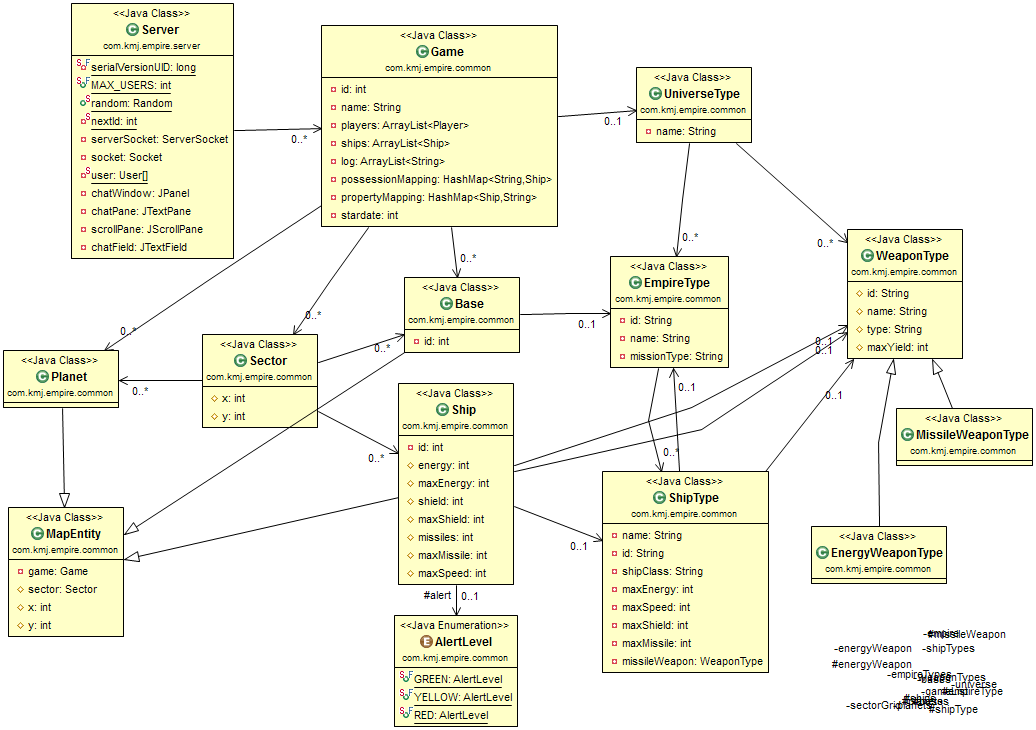
\includegraphics[width=6.5in]{image/domain_model_img}
\end{figure}

\section{Links}
\begin{description}
	\item[Unit Test Screencast] https://www.youtube.com/watch?v=NFcnP\_zS7xA\&feature=youtu.be
	\item[Unit Test] https://github.com/mdclyburn/empire-game/tree/\\server/src/com/kmj/empire/server/JUnitTestServer.java
	\item[Domain Model Classes] https://github.com/mdclyburn/empire-game/\\tree/server/src/com/kmj/empire/common
	\item[Restore Game] https://github.com/mdclyburn/empire-game/tree/\\server/src/com/kmj/empire/server/GameServiceImpl.java
\end{description}

\section{Unit Test}
\begin{enumerate}
	\item Change directory into the local repository.
	\item Checkout the 'server' branch with:\\
	\begin{center}
	'git checkout server'
	\end{center}
	\item Compile source with:\\
	'javac -cp src:lib/gson.jar:lib/junit.jar src/com/kmj/empire/server/*.java\\
	src/com/kmj/empire/common/*.java'
	\item Start the server with:\\
	'java -cp src:lib/gson.jar com.kmj.empire.server.Server'
	\item Start the unit test with:\\
	'java -cp src:lib/gson.jar:lib/junit.jar:lib/hamcrest.jar org.junit.runner.JUnitCore\\
	com.kmj.empire.server.JUnitTestServer'
\end{enumerate}
